%
% interpolacao.tex (LateX)
% 
% Objetivo: Capítulo sobre a etapa de interpolação do relatório de qualificação de doutorado.
% 
% Versão 1.0
% 
% Site: http://www.dirackslounge.online
% 
% Programador: Rodolfo A. C. Neves (Dirack) 17/10/2019
% 
% Email: rodolfo_profissional@hotmail.com
% 
% Licença: GPL-3.0 <https://www.gnu.org/licenses/gpl-3.0.txt>.

\chapter{INTERPOLAÇÃO COM FILTROS ADAPTATIVOS DE PREDIÇÃO DE ERRO}
\label{cap6:interpolacao}

A intepolação com FPE permite aumentar a amostragem dos dados modelados (vide Capítulo \ref{cap5:modeling}),
de 401 PMC's para 802.
e diminuir a discretização, de 0.025Km para 0.0125Km na distância entre os PMC's.
Isto permite amostrar adequadamente as famílias ERC, com os traços da família o mais próximo possível
das coordenadas $m$, $h$ da trajetória ERC calculada a partir da Equação \ref{eq:2.1}.

Obviamente, poderíamos ter realizado a etapa de modelagem com uma discretização maior. 
Porém, o intuito deste experimento é demonstrar como
a intepolação com FPE pode regularizar a amostragem dos dados, possibilitando a busca pelos
traços sobre as trajetórias ERC com a maior precisão possível.

Antes da interpolação, os traços nas coordenadas $m$ e $h$ são separados em seções de afastamento constante, 
cada uma com 401 PMC's.
A interpolação com os filtros adaptativos de predição de erro (FPE) é realizada para cada seção em duas etapas,
como descrito no Capítulo \ref{cap4:pef}:

\begin{enumerate}
 \item Intercalamos traços zerados com os traços originais da seção e calculamos os coeficientes do FPE
 com auxílio da Equação \ref{eq:4.1}.
 
 \item Interpolamos os traços zerados utilizando os traços originais como restrição (Equações \ref{eq:4.9}-\ref{eq:4.10}).
\end{enumerate}

O raio da janela de suavização do filtro no espaço e no tempo e a quantidade de coeficientes do filtro no espaço e no
tempo para cada amostra são determinados por tentativa e erro: Selecionamos uma seção de afastamento constante, realizamos a
etapa de interpolação diversas vezes para determinar os valores destes parâmetros. 
Os valores escolhidos que produziram os melhores resultados na interpolação
foram 10 coeficientes no tempo e 2 no
espaço para cada amostra; e 50 amostras no tempo e 2 amostras no espaço,
como raio da janela de suavização gaussiana do FPE.

Após esta etapa, calculamos as trajetórias ERC para cada $m0$, no intervalo $5Km<m_0<6Km$ com amostragem
$\delta m_0 = 0.0125Km$; e para cada $t_0$, no intervalo $1s<t_0<2s$, com mostragem $\delta t_0 = 0.004s$.
Estes pares $m_0, t_0$ serão os pontos da malha da seção empilhada ERC.
Determinamos as coordenadas $m$, $h$ da trajetória ERC que intersectam as seções de afastamento constante com
auxílio da Equação \ref{eq:2.1}.
Estes pontos são as coordendas dos traços que pertencem à trajetória ERC, por definição.

Por fim, buscamos nas seções interpoladas
os traços sísmicos mais próximos das coordenadas calculadas anteriormente, estes traços formam as famílias ERC. 
Cada par $m0, t_0$ possuirá uma família ERC, parâmetros $R_N$, $R_{NIP}$ e $\beta_0$ e também terá uma curva de tempo
de trânsito ERC correspondente (calculada a partir da Equação \ref{eq:2.3}) sobre a qual será realizado o empilhamento.

O empilhamento ERC é realizado sobre as curvas de tempo de trânsito ERC, somando as amplitudes
das amostras sobre a curva nas seções ERC e atribuindo esta soma aos pares $m0$, $t0$ na seção empilhada ERC.
Fazendo isto para todos os pontos dá malha, a imagem da seção empilhada ERC é formada.

As Figuras \ref{fig:6.1}-\ref{fig:6.2} apresentam algumas seções ERC organizadas pela coordenada do afastamento $h$. A Figura
\ref{fig:6.1} é a seção ERC para o $m0=5Km$ e as Figuras \ref{fig:6.2}-\ref{fig:6.3} para o $m0=4Km$. O ajuste feito com
a equação de tempo de trânsito ERC (pontos em amarelo) depende da escolha correta do tempo $t0$ e dos parâmetros
$R_N$, $R_{NIP}$ e $\beta_0$. 

Na Figura \ref{fig:6.3}, 
o $t0=1.1s$ utilizado não é apropriado, não produzindo o melhor ajuste com o evento de reflexão.
O empilhamento sobre estas curvas tende a produzir somas destrutivas, enquanto o empilhamento
sobre curvas de melhor ajuste, como no caso da Figura \ref{fig:6.2},
tendem a ressaltar os eventos de reflexão na seção empilhada e a suprimir o ruído aleatório.

\begin{figure}
\caption{Seção ERC para o PMC $m0=5Km$ e $t0=1.1s$.
Pontos em amarelo representam a curva de tempo de trânsito ERC sobre a qual
é realizado o empilhamento.
O eixo horizontal é a coordenada do afastamento $h$ e o eixo vertical o tempo
$t$.}
\begin{center}
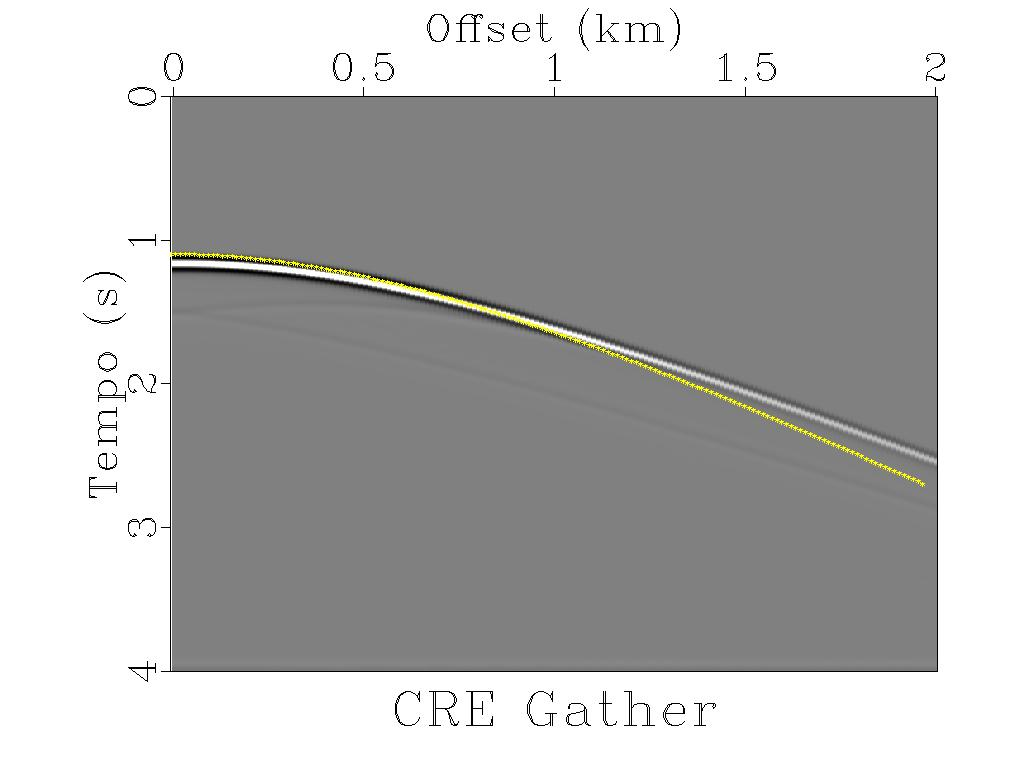
\includegraphics[scale=0.3]{images/interpolacao5.jpeg}
\vspace{-0.3cm}
\end{center}
\begin{center}
 Fonte: Do Autor.
\end{center}
\label{fig:6.1}
\end{figure}

\begin{figure}
\caption{Seção ERC para o PMC $m0=4Km$ e $t0=1.3s$.
Pontos em amarelo representam a curva de tempo de trânsito ERC sobre a qual
é realizado o empilhamento ERC.
O eixo horizontal é a coordenada do afastamento $h$ e o eixo vertical o tempo
$t$.}
\begin{center}
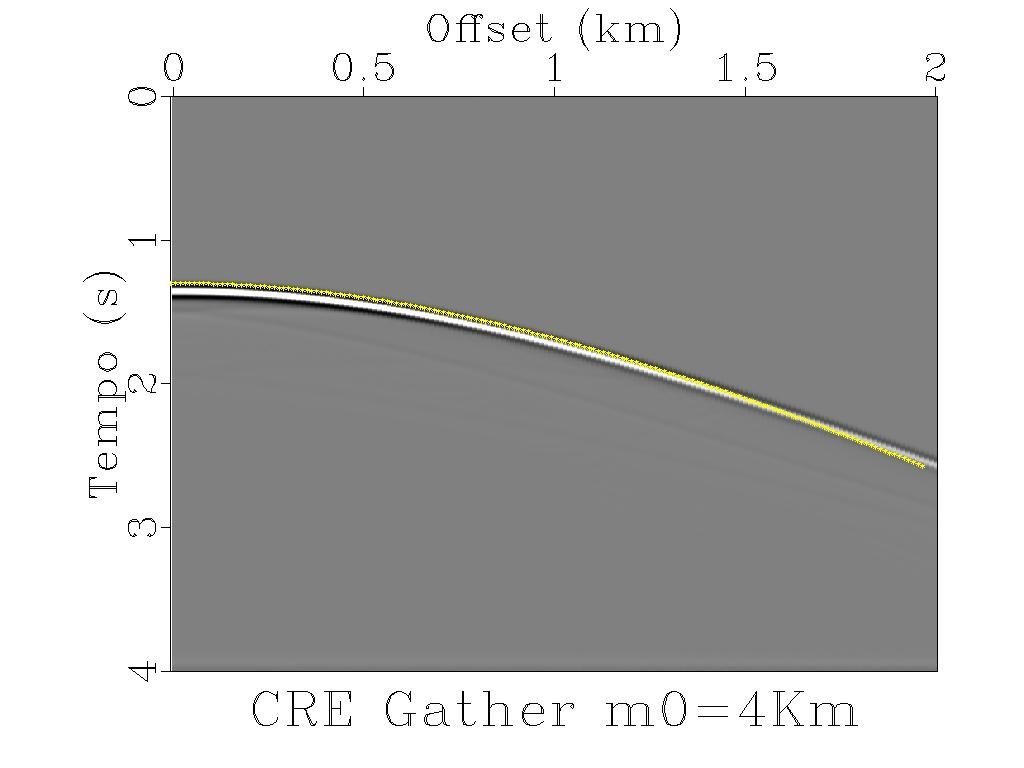
\includegraphics[scale=0.3]{images/interpolacao4.jpeg}
\vspace{-0.3cm}
\end{center}
\begin{center}
 Fonte: Do Autor.
\end{center}
\label{fig:6.2}
\end{figure}

\begin{figure}
\caption{Seção ERC para o PMC $m0=4Km$ e $t0=1.1s$.
Pontos em amarelo representam a curva de tempo de trânsito ERC sobre a qual
é realizado o empilhamento ERC.
O eixo horizontal é a coordenada do afastamento $h$ e o eixo vertical o tempo
$t$. A escolha de $t0=1.1$ não produziu o melhor ajuste da curva ERC aos dados modelados.}
\begin{center}
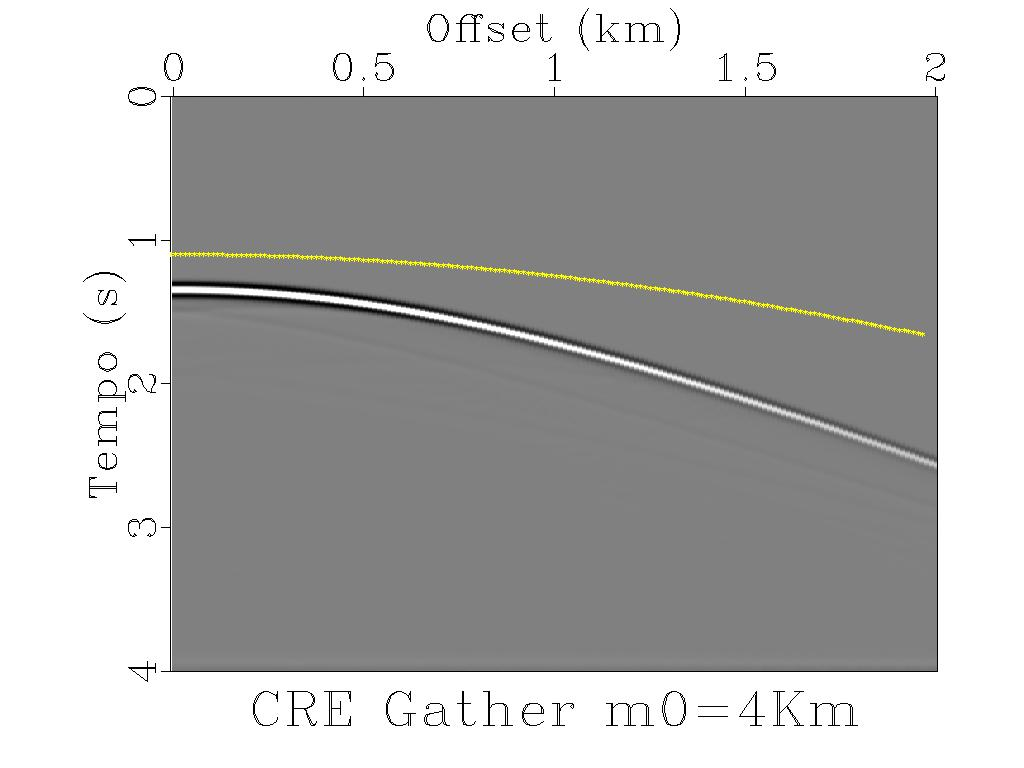
\includegraphics[scale=0.3]{images/interpolacaoErro.jpeg}
\vspace{-0.3cm}
\end{center}
\begin{center}
 Fonte: Do Autor.
\end{center}
\label{fig:6.3}
\end{figure}
